\documentclass{article}

\title{The Writeup of Assignment 4 - Multithread HTTP server}

\author{Dongjing Wang}

\date{December 06, 2022}

\usepackage{graphicx}

\begin{document}
\maketitle

\section{Design}
    \begin{figure}[htbp]
        \centering
        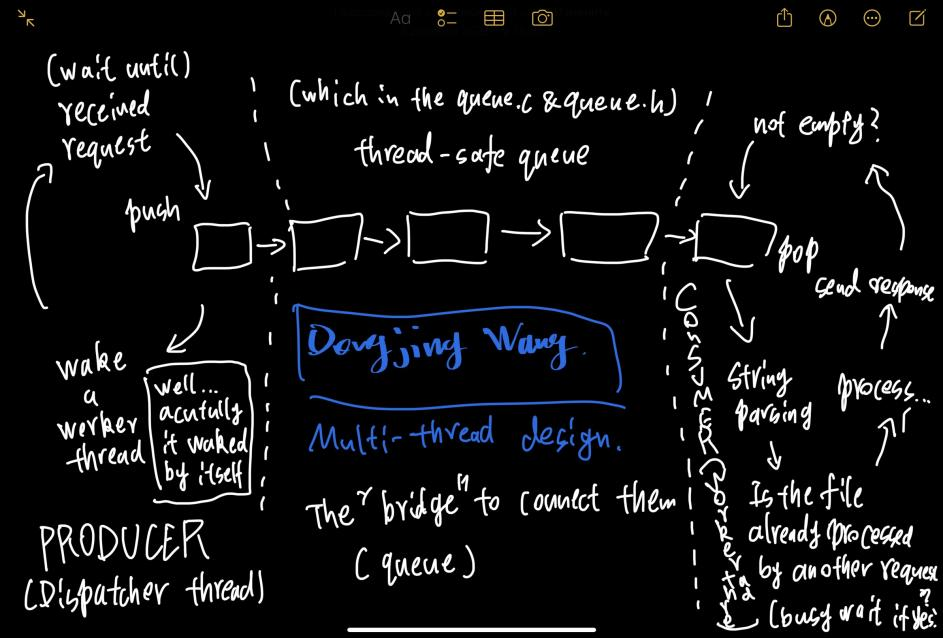
\includegraphics[width=1.1\textwidth]{IMG_0066.jpg}
        \caption{The basic design of my multithread server}
        \label{fig:design}
    \end{figure}
    The main design idea is as shown in the figure. There are three main parts of the whole program, namely PRODUCER, thread-safe queue, CONSUMER. Let me introduce these three parts one by one.
    \subsection{PRODUCER}
        As shown in the figure, PRODUCER can be understood as working in a loop all the time. That's why I put it in a for loop and keep running. I've been thinking about how to make both the PRODUCER and CONSUMER run in an infinite loop but independently of each other. The solution that I thought of later was to put CONSUMER in the for loop to create those threads (which is actually equivalent to running all the time), and put Producer in while(1) to keep running. In this cycle, there are three parts that together make up this cycle.
        \subsubsection{Receive request}
            This part is mainly related to the function in \textbf{bind.c}, the accept in the main function and calling \textbf{create\_listen\_socket} to connect port and socket.
        \subsubsection{push}
            This part is mainly composed of the queue structure in \textbf{queue.c}. It is a queue capable of working in a multi-threaded environment. But it is different from the queue I wrote before. Since the queue I wrote before has not been able to work perfectly in a multi-threaded environment, I transferred the \textbf{pthread cond init} and \textbf{pthread cond signal} to the main file. Then it should work mostly fine. The difference between this queue and the ordinary thread queue is that when the queue is empty or full, pop and push will not simply return failure but will enter busy waiting until the condition is no longer satisfied and then executed. Another point is that when the push and pop functions try to change the queue, they will lock the queue and prevent other threads from entering the critical region.
        \subsubsection{wake a worker thread}
            This part can be understood as "wake up the worker thread", but in fact the worker thread just enters the busy waiting state. It has been waiting to see if the queue is still empty. When the queue is no longer empty (that is, after the dispatcher thread puts something in), they will automatically start working.
    \subsection{Queue}
        The content of the queue is basically in \textbf{queue.c} and \textbf{queue.h}. They are mainly used to connect PRODUCER and CONSUMER. This allows PRODUCER and CONSUMER to work independently and communicate with each other.
    \subsection{CONSUMER}
        CONSUMER can also be understood as a cycle, but it is more complicated than PRODUCER.
        \subsubsection{pop}
            When the queue is no longer empty, the worker thread will automatically pop out the contents and try to proceed to the next step, which is string parsing.
        \subsubsection{string parsing}
            I've already used string parsing when experimenting with single-threaded servers. But at that time, the test script provided was rather strange (it will send a string of binary stuff to my server in order to test whether it is connected. Since I did not use regex but strtok\_r, this will cause segmentation fault). But now I don't need to think about this issue, and I will delete the hard coding for this part. It is still the same as before: first separate them according to the URL line, header field, and message body. Then get the method and path from the URL line. And check whether there is "Request -Id" as the key in the header field. Read the following value, if any.
        \subsubsection{Accessing files}
            After string parsing, we get all the information we need. The next step is to try the access file. Since we cannot allow two threads to enter the critical region at the same time - that is, the file. So I created \textbf{filelinkedlist.c} and \textbf{filelinkedlist.h}. The newly created linked list here can be understood as a set. When the thread is about to start accessing the file, it will try to insert the file name (path) into the linked list. If there is already a duplicate (that is, other threads are accessing this file), it will enter a waiting state until another thread completes processing and deletes the file name (path).
        \subsubsection{process \& send response}
            After successfully entering the file, the next thing to do is to perform different operations on the file according to different methods. After completing the operation, you need to put the corresponding \textit{method, path, status code, request id} into the audit log. This also needs to be noticed, because this is also a critical region. So I used flock to deal with this situation. What needs to be done after this step is to send the response to the client.
        \subsubsection{checking}
            After the previous step is completed, this step is basically equivalent to the beginning of the next cycle. What the thread has to do in this step is to wait. When the queue is no longer empty and no other threads have popped out, it will start a new round of work...
\section{Conclusion}
    I learned a lot in class, but I couldn't really understand it because of my ability. After combining the homework, I found that many "illusory" concepts in the class are actually the crystallization of the wisdom of computer scientists. Since I was in strike at the time, there was no tutor or TA to help me. I don't know many people, so I don't have many friends with whom to discuss this issue. So sometimes I reserve a room in the library and work on the whiteboard myself.
    \begin{figure}[htbp]
        \centering
        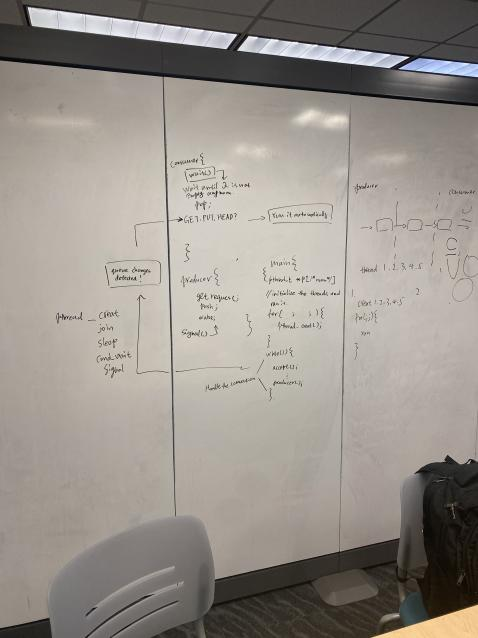
\includegraphics[width=0.5\textwidth]{IMG_1179.jpg}
        \caption{The design before coding in S\&E}
        \label{fig:design}
    \end{figure}
    When I was in CSE 13S, the professor said that design is extremely important for programmers, but I didn't understand it. Until I tried to change what was once a single-threaded server without design and I was frustrated by the increasing complexity. Later, I decided to study the design alone and control the entry of my coding before the design was completed, and this is the reason why I can make the multi-threaded server what it is now (although it is not perfect). But I learned a lot.
\end{document}